\section{はじめに}
拡散モデル~\cite{song2021score,karras2022edm}は,学習済みのモデルを凍結したまま分布外検知に使える. 尤度や統計量による方法~\cite{serra2020input,mahmood2021msma,heng2024diffpath,alexis2026gepc,shoushtari2026eigenscore}は, 1枚あたり10回から数百回のネットワークの評価を要する. CFS~\cite{rouzoumka2026cfs}は低いノイズでの1回の順伝播から中間特徴~\cite{xiang2023ddae}を読んでこれらを上回るが, 1{,}024次元の特徴を学習画像5万枚の統計量や近傍と比べる.

\begin{figure*}[t]\centering
\begin{adjustbox}{max width=\textwidth}% fig_method.tex -- Figure 1: the method in pictures (TikZ, drawn by hand; absolute coordinates in cm, natural width about 18.7 cm).
%   (a) test time: the image goes through the frozen U-Net up to block A (the pass stops there); of every block ONE number is read (the
%       amplitude: per channel the largest deviation from the spatial mean, log, mean over channels).  The numbers form the profile.  The
%       score is one Mahalanobis distance: from the profile to the point mu*.
%   (b) once, before: the n held-out ID images in the eight orientations of the square.  As they are: mean mu and covariance S of the
%       profile.  The seven other orientations: the mean mu_o.  No feature of a training image is stored.
%   (c) what the score means: mu* is mu moved away from mu_o; a profile on the mu_o side is far from mu*.
%   Colours: black, navy (ID side), red (the test image / what is computed).  The curves and the layout of (c) are a schematic, not data.
\begin{tikzpicture}[font=\scriptsize, >={Stealth[length=1.5mm, width=1.2mm]}, line join=round, line cap=round,
  lab/.style={font=\tiny, inner sep=1pt, align=center}, ttl/.style={font=\scriptsize, anchor=south west, inner sep=0pt}]
\def\unet#1#2#3#4#5{% origin (left block, centre height), scale, style of the down path and bottom, style of block A, style of the rest of the up path
  \begin{scope}[shift={#1}, scale=#2]
    \foreach \dx/\yc/\h in {0/0/1.5, 0.3/0/1.5, 0.75/-0.5/1.0, 1.05/-0.5/1.0, 1.5/-0.95/0.6, 1.8/-0.95/0.6, 2.25/-0.95/0.6, 2.55/-0.95/0.6}
      \draw[#3] (\dx,\yc-\h/2) rectangle ++(0.22,\h);
    \draw[#4] (3.2,-1.0) rectangle ++(0.22,1.0);
    \foreach \dx/\yc/\h in {3.5/-0.5/1.0, 3.95/0/1.5, 4.25/0/1.5}
      \draw[#5] (\dx,\yc-\h/2) rectangle ++(0.22,\h);
    \draw[#3] (0.52,0) -- (0.75,-0.5) (1.27,-0.5) -- (1.5,-0.95) (2.02,-0.95) -- (2.25,-0.95) (2.77,-0.95) -- (3.2,-0.5);
    \draw[#5] (3.72,-0.5) -- (3.95,0);
  \end{scope}}
%% ================================================================ (a) test time
\node[ttl] at (0,0.3) {\textbf{(a)}\ テスト時：ブロックAまで通し,ブロックごとに数値を1つだけ読む};
\node[inner sep=0, draw=black!60] at (0.62,-1.0) {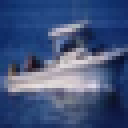
\includegraphics[width=1.0cm]{figs/ex_id.png}};
\node[lab, anchor=north] at (0.62,-1.57) {テスト画像 $\vec{x}$};
\draw[->] (1.16,-1.0) -- node[above, lab] {$+\sigma_1\veps$} (1.84,-1.0);
\unet{(1.9,-1.0)}{1}{black, line width=0.7pt}{redc, fill=redc!35, line width=0.9pt}{black!40, densely dashed, line width=0.5pt}
\node[lab, anchor=south west] at (1.9,-0.2) {ノイズ除去器(U-Net, 凍結). 順伝播は1回};
\node[lab, anchor=north west, text=redc] at (5.02,-2.03) {\textbf{ブロックA}で止める};
\draw[black!70, decorate, decoration={brace, mirror, amplitude=3pt}] (1.9,-2.42) -- (5.32,-2.42);
\node[lab, anchor=north] at (3.6,-2.55) {ブロックAまでの出力};
% ---- the amplitude of one block: one channel, the largest deviation from its spatial mean
\draw[->] (6.5,-1.0) -- (7.2,-1.0);
\foreach \i/\j/\s in {0/0/12,1/0/20,2/0/8,3/0/15,4/0/10, 0/1/18,1/1/10,2/1/25,3/1/12,4/1/8, 0/2/8,1/2/15,2/2/12,3/2/90,4/2/20, 0/3/14,1/3/8,2/3/18,3/3/22,4/3/10, 0/4/10,1/4/16,2/4/9,3/4/13,4/4/17}
  \fill[black!\s] ({7.3+0.26*\i},{-0.55-0.26*\j}) rectangle ++(0.26,-0.26);
\draw[black!60] (7.3,-0.55) rectangle (8.6,-1.85);
\draw[redc, line width=1.0pt] (8.08,-1.07) rectangle ++(0.26,-0.26);
\node[lab, anchor=south] at (7.95,-0.52) {ブロック $h$ の1チャネル};
\node[lab, anchor=north, text=redc] at (7.95,-1.88) {平均から最も離れた値};
\node[lab, anchor=north] at (7.95,-2.2) {その大きさの対数を\\チャネルで平均};
\draw[->] (8.7,-1.2) -- node[above, lab] {$a_h(\vec{x})$} node[below, lab] {数値1つ} (9.75,-1.2);
% ---- the profile: one number per block up to A
\draw[black!45, rounded corners=3pt] (9.8,-0.2) rectangle (14.25,-3.15);
\draw[->, black!80] (10.25,-2.8) -- (14.1,-2.8); \draw[->, black!80] (10.25,-2.8) -- (10.25,-0.4);
\node[lab, anchor=north east] at (14.15,-2.84) {ブロック $h$};
\node[lab, anchor=south west] at (10.3,-0.62) {振幅 $a_h$};
\fill[navyc!18] (10.5,-1.75) -- (11.0,-1.45) -- (11.5,-1.6) -- (12.0,-1.25) -- (12.5,-1.0) -- (13.0,-1.35) -- (13.5,-1.15) -- (13.95,-1.45)
  -- (13.95,-1.95) -- (13.5,-1.65) -- (13.0,-1.85) -- (12.5,-1.5) -- (12.0,-1.75) -- (11.5,-2.1) -- (11.0,-1.95) -- (10.5,-2.25) -- cycle;
\draw[navyc, line width=0.9pt] (10.5,-2.0) -- (11.0,-1.7) -- (11.5,-1.85) -- (12.0,-1.5) -- (12.5,-1.25) -- (13.0,-1.6) -- (13.5,-1.4) -- (13.95,-1.7);
\draw[black, densely dashed, line width=0.8pt] (10.5,-1.75) -- (11.0,-1.4) -- (11.5,-1.5) -- (12.0,-1.05) -- (12.5,-0.75) -- (13.0,-1.15) -- (13.5,-0.9) -- (13.95,-1.15);
\draw[redc, line width=1.0pt] (10.5,-2.2) -- (11.0,-2.05) -- (11.5,-2.4) -- (12.0,-2.0) -- (12.5,-2.1) -- (13.0,-1.95) -- (13.5,-2.25) -- (13.95,-2.3);
\foreach \p in {(10.5,-2.2),(11.0,-2.05),(11.5,-2.4),(12.0,-2.0),(12.5,-2.1),(13.0,-1.95),(13.5,-2.25),(13.95,-2.3)} \fill[redc] \p circle (0.05);
\node[lab, anchor=south, text=redc] at (13.95,-0.75) {A};
\draw[black!55, densely dotted] (13.95,-2.8) -- (13.95,-0.78);
\node[lab, anchor=west] at (10.42,-0.95) {$\vmu^{*}$(破線)};
\node[lab, anchor=west, text=navyc] at (11.75,-0.62) {分布内の画像($\vmu$ と幅)};
\node[lab, anchor=west, text=redc] at (10.42,-2.62) {テスト画像 $\va(\vec{x})$};
\draw[<->, redc, line width=0.5pt] (12.5,-0.8) -- (12.5,-2.05);
% ---- one distance -> the score
\draw[->] (14.35,-1.6) -- (14.85,-1.6);
\node[draw=black, rounded corners=2pt, line width=0.9pt, inner sep=3pt, align=center, font=\tiny, text width=20mm] at (16.1,-1.6) {$\vmu^{*}$ までの\\マハラノビス距離\\(式は1つ)};
\draw[->] (17.3,-1.6) -- (17.75,-1.6);
\node[lab, anchor=west] at (17.72,-1.6) {$s(\vec{x})$};
\node[lab, anchor=north, text=black!60] at (16.1,-2.3) {近いほど分布内};
%% ================================================================ (b) prepared once
\node[ttl] at (0,-3.95) {\textbf{(b)}\ 事前の準備(1回だけ)：分布内の画像\olNRefMax{}枚を8つの向きで通す};
\node[inner sep=0, draw=navyc, line width=0.8pt] at (0.5,-5.0) {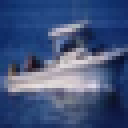
\includegraphics[width=0.62cm]{figs/ex_id.png}};
\node[lab, anchor=north, text=navyc] at (0.5,-5.36) {そのまま};
\foreach \x/\y/\r/\sx/\sy in {1.55/-4.72/0/1/-1, 2.3/-4.72/0/-1/1, 3.05/-4.72/180/1/1, 3.8/-4.72/90/1/1, 1.55/-5.52/270/1/1, 2.3/-5.52/90/1/-1, 3.05/-5.52/270/1/-1}
  \node[inner sep=0, rotate=\r, xscale=\sx, yscale=\sy] at (\x,\y) {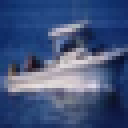
\includegraphics[width=0.62cm]{figs/ex_id.png}};
\node[lab, anchor=west] at (3.45,-5.52) {残り7つの向き};
\draw[->] (4.7,-5.1) -- (5.15,-5.1);
\unet{(5.25,-4.95)}{0.3}{black, line width=0.35pt}{redc, fill=redc!35, line width=0.35pt}{black!40, densely dashed, line width=0.3pt}
\draw[->] (6.7,-5.1) -- (7.15,-5.1);
\pgfmathsetseed{7}
\foreach \i in {1,...,12} {\pgfmathsetmacro{\sa}{0.2*(rnd-0.5)}\pgfmathsetmacro{\sb}{0.2*(rnd-0.5)}\pgfmathsetmacro{\sc}{0.2*(rnd-0.5)}\pgfmathsetmacro{\sd}{0.2*(rnd-0.5)}\pgfmathsetmacro{\se}{0.2*(rnd-0.5)}
  \draw[navyc!55, line width=0.3pt] (7.3,{-4.85+\sa}) -- (7.7,{-4.55+\sb}) -- (8.1,{-4.7+\sc}) -- (8.5,{-4.3+\sd}) -- (8.9,{-4.5+\se});}
\foreach \i in {1,...,12} {\pgfmathsetmacro{\sa}{0.2*(rnd-0.5)}\pgfmathsetmacro{\sb}{0.2*(rnd-0.5)}\pgfmathsetmacro{\sc}{0.2*(rnd-0.5)}\pgfmathsetmacro{\sd}{0.2*(rnd-0.5)}\pgfmathsetmacro{\se}{0.2*(rnd-0.5)}
  \draw[black!45, line width=0.3pt] (7.3,{-5.75+\sa}) -- (7.7,{-5.6+\sb}) -- (8.1,{-5.85+\sc}) -- (8.5,{-5.6+\sd}) -- (8.9,{-5.8+\se});}
\draw[->, navyc, line width=0.9pt] (9.1,-4.6) -- (9.6,-4.6);
\node[lab, anchor=west, text=navyc] at (9.62,-4.6) {平均 $\vmu$,共分散 $\Sm$};
\draw[->, black!70, line width=0.9pt] (9.1,-5.7) -- (9.6,-5.7);
\node[lab, anchor=west] at (9.62,-5.7) {平均 $\vmu_{o}$};
\node[lab, anchor=west] at (0.1,-6.35) {保存するのは $\vmu^{*}$ と $(\Sm+\lambda\bar{s}\Id)^{-1}$ の計\olNStored{}個の数値(CIFAR-10). 勾配による学習も,学習画像の特徴の保存もない};
%% ================================================================ (c) what the score means
\node[ttl] at (12.2,-3.95) {\textbf{(c)}\ スコアの意味};
\draw[black!45, rounded corners=3pt] (12.2,-4.15) rectangle (18.7,-6.55);
\draw[black!55, fill=black!10, rotate around={25:(13.35,-5.85)}] (13.35,-5.85) ellipse (0.62 and 0.3);
\draw[navyc, fill=navyc!18, rotate around={25:(15.0,-5.2)}] (15.0,-5.2) ellipse (0.62 and 0.3);
\foreach \a/\b in {1.25/0.6, 2.05/0.98} \draw[redc!70, densely dashed, line width=0.4pt, rotate around={25:(17.2,-4.33)}] (17.2,-4.33) ++(180:\a) arc[start angle=180, end angle=290, x radius=\a, y radius=\b];
\draw[black!70, line width=0.5pt] (13.35,-5.85) -- (15.0,-5.2);
\draw[->, redc, line width=0.8pt] (15.0,-5.2) -- (17.13,-4.36);
\fill[black!70] (13.35,-5.85) circle (0.05); \fill[navyc] (15.0,-5.2) circle (0.05); \fill[redc] (17.2,-4.33) circle (0.06);
\node[lab, anchor=north] at (13.35,-6.18) {向きを変えた画像};
\node[lab, anchor=south east] at (13.3,-5.8) {$\vmu_{o}$};
\node[lab, anchor=west, text=navyc] at (15.62,-5.38) {分布内の画像};
\node[lab, anchor=south east, text=navyc] at (15.0,-5.15) {$\vmu$};
\node[lab, anchor=west, text=redc] at (17.27,-4.33) {$\vmu^{*}$};
\node[lab, anchor=south east, text=redc] at (16.25,-4.62) {$c(\vmu-\vmu_{o})$};
\fill[redc] (14.35,-6.05) circle (0.045); \draw[redc, line width=0.4pt, densely dotted] (14.35,-6.05) -- (17.2,-4.33);
\node[lab, anchor=west, text=redc] at (14.45,-6.2) {テスト画像のプロファイル};
\node[lab, anchor=east, text=black!60] at (18.6,-6.3) {破線：スコアが等しい線};
\end{tikzpicture}
\end{adjustbox}
\caption{\Ours{}の概要. (a) テスト時：ブロックAまで通し,ブロックごとの振幅[式~\eqref{eq:amp}]の並びから点 $\vmu^{*}$ までのマハラノビス距離をスコアとする. (b) 事前の準備：分布内の画像を8つの向きで通し, $\vmu$, $\Sm$, $\vmu_{o}$ を求める. (c) $\vmu^{*}$ は $\vmu$ を $\vmu_{o}$ の反対側へ動かした点で, $\vmu_{o}$ の側へ外れた並びほど遠い. 折れ線と配置は模式図である.}
\label{fig:method}
\end{figure*}

本研究の\Ours{}は, U-Net~\cite{ronneberger2015unet}のブロックごとに数値を1つ(振幅)だけ読み,その並びを1つの式で判定する(図~\ref{fig:method}). 学習済みのモデルの振幅は,分布外の画像で下がることが多い(\ref{sec:fall}節). この下がる方向を,分布外の画像を使わずに,分布内の画像の向きを変えて求める. 上下反転や回転をした画像は,画素の値の集まりが同じまま見慣れない画像になり,振幅が下がるからである. スコアは,分布内の平均をこの方向の反対側へ動かした点へのマハラノビス距離~\cite{lee2018mahalanobis}である. 勾配による学習,追加のネットワーク,人手のラベル,分布外の画像は使わない.

5つの分布内データセットで,自然画像の分布外集合に対する平均AUROCは test で\olTestOL\%で,先行研究の最良(\olBestPriorName, \olBestPriorMean\%)を\olGapCfsKnn{}ポイント上回った(95\%信頼区間[\olGapCfsKnnLo, \olGapCfsKnnHi]). 6つのテスト分割では\olSixMin{}〜\olSixMax\%であった. 順伝播は途中で止める1回で, CPUで1枚\olSecOL{}秒(途中で止めたCFSの\olSecRatioCfsKnn{}倍),保存する数値は\olNStored{}個である. 縮小の履歴をそろえた対照でもCFSとの差は変わらず,重みを初期化したままにすると\olVarRinit\%に下がる. 一方, $256{\times}256$ のImageNetでは向きを変えても並びがほとんど動かず,方向の手がかりは働かない(上下反転は\olHrOLVf\%). なお,定数1つ($c=8$)は開発用の分割で決め,テスト分割は以前に他の手法で結果を見たものである.

\section{先行研究}
\label{sec:related}
\textbf{尤度と統計量.} 深層生成モデルは分布外の画像に高い尤度を与えることがある~\cite{nalisnick2019deep,serra2020input}. これを補う典型集合の検定~\cite{nalisnick2019typ},入力の複雑さによる補正~\cite{serra2020input},スコアの大きさ~\cite{mahmood2021msma},生成の軌跡~\cite{heng2024diffpath},事後平均の一貫性~\cite{alexis2026gepc},事後共分散~\cite{shoushtari2026eigenscore},内在次元~\cite{kamkari2024geometric}は,多くが1枚あたり10回以上のネットワークの評価を要する.

\textbf{中間特徴.} kNN~\cite{sun2022knn}は学習画像の特徴への近さで, SSD~\cite{sehwag2021ssd}は特徴のまとまりへのマハラノビス距離~\cite{lee2018mahalanobis}で判定する. CFS~\cite{rouzoumka2026cfs}は拡散モデルの2つのブロックの出力をチャネルごとの平均と標準偏差にまとめ,対角の正規分布や近傍で判定する. MSMA~\cite{mahmood2021msma}はノイズの大きさごとのスコアの大きさを並べ,分布内の密度を当てはめる. \Ours{}が並べるのはブロックごとの振幅で,外れのうち振幅が下がる方向を重く数える.

\textbf{特徴の大きさ.} 分類器では,中間特徴のノルムが分布外の画像で小さくなる~\cite{yu2023featurenorm,park2023featurenorm}. これらは分布内のラベルで学習した分類器を要し, FeatureNorm~\cite{yu2023featurenorm}は読むブロックを擬似的な分布外の画像で選ぶ. \Ours{}はラベルなしで学習した拡散モデルを使い,ブロックは解像度だけで決める.

\textbf{変換した画像と背景の分布.} 回転の予測~\cite{gidaris2018rotnet}で学習した分類器を使う方法~\cite{golan2018geometric,hendrycks2019ss},回転した分布内の画像を対照学習の負例にするCSI~\cite{tack2020csi},補助の分布外データで学習するOutlier Exposure~\cite{hendrycks2019oe},背景のモデルとの尤度比~\cite{ren2019likelihood},相対マハラノビス距離~\cite{ren2021simple}がある. GEPC~\cite{alexis2026gepc}は,変換した入力に対するノイズ除去器の出力の一貫性を14回の評価で測る. \Ours{}は向きを変えた分布内の画像を学習に使わず,凍結したモデルでの並びの平均を1つ求めるためだけに使う.

\section{提案手法：\Ours}
\label{sec:method}
\textbf{問題設定.} 拡散モデルのノイズ除去器と,評価に用いない分布内の画像 $\vec{x}_1,\dots,\vec{x}_n$(val1. \olNRefMin{}〜\olNRefMax{}枚)だけを用いる. テスト画像 $\vec{x}$ に,分布内の画像ほど大きいスコア $s(\vec{x})$ を与える.

\subsection{振幅の並び}
\label{sec:amp}
画像 $\vec{x}$ にノイズ $\sigma_1\veps$($\sigma_1=0.01$. $\veps$ は全画像に共通)を加えてノイズ除去器に通す. ブロック $h$ の出力の,チャネル $c$,位置 $u$ での値を $f_{h,c,u}(\vec{x})$,チャネルの数を $C_h$,位置の数を $U_h$ とし,チャネルごとの空間平均を
\begin{equation}
\bar{f}_{h,c}(\vec{x})=\frac{1}{U_h}\sum_{u=1}^{U_h}f_{h,c,u}(\vec{x})
\label{eq:fbar}
\end{equation}
とする. ブロック $h$ の振幅を
\begin{equation}
a_h(\vec{x})=\frac{1}{C_h}\sum_{c=1}^{C_h}\log\max_{u}|f_{h,c,u}(\vec{x})-\bar{f}_{h,c}(\vec{x})|
\label{eq:amp}
\end{equation}
と定める. チャネルごとに空間平均から最も離れた値を見る量で,どこかに強い応答があれば大きい. デコーダで出力が $16{\times}16$ になる最初のブロックをAとし(5つのモデルで同じ規則. 補足資料の表~\ref{tab:models}),入力からAまでの $p$ 個の振幅を並べた
\begin{equation}
\va(\vec{x})=\{a_1(\vec{x}),\dots,a_p(\vec{x})\}
\label{eq:profile}
\end{equation}
をプロファイルと呼ぶ(CIFAR-10で $p=\olNBlkCten$). 順伝播はAで止めてよい.

\subsection{向きを変えた分布内の画像}
\label{sec:orient}
正方形の画像の向きの変え方は,そのままを除いて7つある(上下反転,左右反転, 180度の回転, 90度と270度の回転, 2本の対角線についての反転). これを $\Gm_1,\dots,\Gm_7$ と書く. どれも画素を並べ替えるだけで,画素の値の集まりは変わらない. 分布内の画像のプロファイルの平均を
\begin{equation}
\vmu=\frac{1}{n}\sum_{i=1}^{n}\va(\vec{x}_i)
\label{eq:mu}
\end{equation}
共分散行列を $\Sm$,向きを変えたときの平均を
\begin{equation}
\vmu_{o}=\frac{1}{7n}\sum_{k=1}^{7}\sum_{i=1}^{n}\va(\Gm_k\vec{x}_i)
\label{eq:muo}
\end{equation}
とする. $\vmu-\vmu_{o}$ は,見慣れた画像が見慣れなくなるときにプロファイルが動く向きの逆である. 7つすべてを使う形は, val2 での開発の8回目の候補である(補足資料A.3).

\subsection{スコア}
\label{sec:score}
分布内の平均を $\vmu_{o}$ の反対側へ動かした点
\begin{equation}
\vmu^{*}=\vmu+c(\vmu-\vmu_{o})
\label{eq:mustar}
\end{equation}
($c=8$. val2 で決めた)と
\begin{equation}
\Pm=(\Sm+\lambda\bar{s}\Id)^{-1}
\label{eq:prec}
\end{equation}
($\bar{s}$ は $\Sm$ の対角成分の平均, $\lambda=10^{-3}$. 分散が0のブロックは除く)を用いて, \Ours{}のスコアを
\begin{equation}
s(\vec{x})=-\{\va(\vec{x})-\vmu^{*}\}^{\top}\Pm\{\va(\vec{x})-\vmu^{*}\}
\label{eq:score}
\end{equation}
とする.

\textbf{2つの項.} 分布内の平均からの距離と,向きの方向への射影を
\begin{equation}
d^{2}(\vec{x})=\{\va(\vec{x})-\vmu\}^{\top}\Pm\{\va(\vec{x})-\vmu\}
\label{eq:dsq}
\end{equation}
\begin{equation}
\ell(\vec{x})=(\vmu-\vmu_{o})^{\top}\Pm\{\va(\vec{x})-\vmu\}
\label{eq:ell}
\end{equation}
とおくと,式~\eqref{eq:score}は
\begin{equation}
s(\vec{x})=-d^{2}(\vec{x})+2c\,\ell(\vec{x})-c^{2}\Delta^{2}
\label{eq:expand}
\end{equation}
と分かれる. $\Delta^{2}=(\vmu-\vmu_{o})^{\top}\Pm(\vmu-\vmu_{o})$ は画像によらない. $-d^{2}$ はどの方向の外れでも小さくなる距離の項, $\ell$ は向きを変えた画像の側へ外れると小さくなる方向の項である. 分布内の画像での $\ell$ の標準偏差はほぼ $\Delta$ なので,向きを変えても並びが動かないデータでは,方向の項は自動的に軽くなる(5つのモデルで $\Delta=\olDeltaMin$〜$\olDeltaMax$).

\textbf{尤度比としての解釈.} 分布内のプロファイルを正規分布 $N(\vmu,\Pm^{-1})$,向きを変えた画像のプロファイルを $N\{\vmu_{o},(1+1/c)\Pm^{-1}\}$ とおくと,
\begin{equation}
\log\frac{N(\va;\vmu,\Pm^{-1})}{N\{\va;\vmu_{o},(1+1/c)\Pm^{-1}\}}=\frac{s(\vec{x})}{2(1+c)}+\mathrm{const.}
\label{eq:llr}
\end{equation}
である(補足資料A.2). ただし,向きを変えた並びの共分散を測ると分布内の\olKapMin{}〜\olKapMax{}倍で(補足資料の表~\ref{tab:kappa}), 1.125倍ではない. $c$ は当てはめた量ではなく, 2つの項の重みである.

\textbf{計算量.} テスト時は,ブロックAで止める順伝播1回(全体の\olFwdAShare\%)と $p$ 次元の2次形式1つである. 保存するのは $\vmu^{*}$ と $\Pm$ の\olNStored{}個の数値(CIFAR-10)で,事前の計算は $8n$ 回の順伝播だけである.

\section{実験}
\label{sec:exp}
\begin{table}[t]\centering\scriptsize\setlength{\tabcolsep}{2.5pt}\renewcommand{\arraystretch}{1.05}
\caption{画像の分け方(9つは互いに重ならない. 分布外データセットは補足資料A.1).}
\label{tab:splits}
\begin{tabular}{@{}l>{\raggedright\arraybackslash}p{0.40\columnwidth}>{\raggedright\arraybackslash}p{0.38\columnwidth}@{}}\toprule
分割 & 画像 & 用途\\\midrule
train & 分布内の学習画像5万枚(ImageNet-64は1万枚) & 比較手法の当てはめ\\[1pt]
val1 & 分布内の画像2{,}000枚(ImageNet-64は1{,}500枚) & \Ours{}の $\vmu$, $\Sm$, $\vmu_{o}$. 比較手法の当てはめ\\[1pt]
val2 & 分布内と各分布外集合から1{,}000枚ずつ(FashionMNISTは2{,}000枚) & \Ours{}の開発(補足資料A.3)\\[1pt]
test & 500枚ずつ & 比較手法との比較(表~\ref{tab:main})\\[1pt]
test2〜6 & 500枚ずつ(test6 のCIFAR-10は\olNCten{}枚) & 分割を変えた確認(表~\ref{tab:six})\\\bottomrule
\end{tabular}
\end{table}
\begin{table*}[t]\centering\scriptsize\setlength{\tabcolsep}{2.6pt}\renewcommand{\arraystretch}{0.88}
\caption{比較手法との比較(AUROC, \%. test). 左の5列：自然画像の分布外集合(分布内ごとに9, 9, 9, 7, 4集合)の平均. 上下反転：上下反転した分布内の画像. 勝/分/負：全\olPairs{}組での\Ours{}の結果(\ref{sec:eval}節. 組ごとの値は補足資料の表~\ref{tab:pairs}). $\dagger$：先行研究の最良. \colorbox{firstblue}{\textbf{水色の太字}}：\Ours{}が最良に並ぶか上回る列.\olUnderlineNote{} 順伝播：1枚あたりの回数(+は逆伝播. $\S$：途中で止める). 秒/枚：CIFAR-10のモデルのCPU時間($\ddagger$：同じ計算機で続けて測定).}
\label{tab:main}
\makebox[\textwidth][c]{\begin{adjustbox}{max width=\textwidth}
\begin{tabular}{@{\hspace{2pt}}lccccc|c|c|c|c|c@{\hspace{2pt}}}\toprule
 & \multicolumn{5}{c|}{分布内(自然画像の分布外集合の平均)} & & & \Ours{}の & & \\
手法 & CIFAR-10 & SVHN & CelebA & ImageNet-64 & FashionMNIST & 5つの平均 & 上下反転 & 勝/分/負 & 順伝播 & 秒/枚\\\midrule
\inputrows{tab_main_ol.tex}
\end{tabular}
\end{adjustbox}}
\end{table*}
\begin{table*}[t]\centering\scriptsize\setlength{\tabcolsep}{3.4pt}\renewcommand{\arraystretch}{0.92}
\caption{6つのテスト分割での\Ours{}(AUROC, \%). 上下反転,左右反転：分布内の画像とその反転を見分けるAUROC. FPR95：\%,低いほどよい. 下の3行は評価の前に登録した変種(6分割の平均). 方向の項：式~\eqref{eq:ell}. 距離の項：式~\eqref{eq:dsq}.}
\label{tab:six}
\begin{adjustbox}{max width=\textwidth}
\begin{tabular}{@{}lccccc|c|c|c|c@{}}\toprule
 & CIFAR-10 & SVHN & CelebA & ImageNet-64 & FashionMNIST & 5つの平均 & 上下反転 & 左右反転 & FPR95\\\midrule
\inputrows{tab_six_ol.tex}
\end{tabular}
\end{adjustbox}
\end{table*}
\subsection{設定}
分布内データセットは5つ(CIFAR-10, SVHN, CelebA, ImageNet-64, FashionMNIST)で,公開されている学習済みの拡散モデルを用いる(FashionMNISTだけは本研究で学習した. 補足資料の表~\ref{tab:models}). 分布外の集合は,他のデータセットの画像(自然画像の分布外集合),上下反転した分布内の画像,合成画像(ImageNet-64と test6 を除く)である. 画像は表~\ref{tab:splits}のように分けた. 比較手法は,同じ拡散モデルを用いる尤度(NLL),入力の複雑さ(IC. PNGとJPEG2000),典型集合の検定(TT), MSMA型, DiffPath, GEPC, EigenScore, CFS(対角ガウスと kNN ヘッド)の\olNPrior{}手法で, test でだけ計算した(補足資料A.1).

\subsection{評価}
\label{sec:eval}
\Ours, CFS, GEPC, EigenScoreはノイズの種3つの平均である. 差の95\%信頼区間は,分布内と分布外の画像を復元抽出するブートストラップ(2{,}000回. 両方の手法に同じ抽出)で求め,信頼区間が0を含まず差が0.05ポイント以上の組を勝ち/負けとする. \Ours{}の式は val2 だけで決め(補足資料A.3),実装を凍結してから6つのテスト分割で1回だけ評価した. 評価の前に書いた主張「6分割の平均が95.0\%以上」は成り立った. ただし,テスト分割はどれも以前に他の手法で結果を見ており,未使用の分割より弱い根拠である. \ref{sec:verify}節の検証と\ref{sec:hrset}節の追加実験は,評価の後に計画を書いてから行った.

\subsection{256{$\times$}256の画像}
\label{sec:hrset}
分布内はImageNetで, ADM~\cite{dhariwal2021adm}の $256{\times}256$ の条件なしモデルを用い,手法とブロックAの規則は変えない. 分布外はOpenOOD v1.5~\cite{zhang2023openood}のSSB-hard, NINCO, iNaturalist, Textures, OpenImage-Oである. すべての画像を224ピクセルにそろえてから拡大し,較正に分布内の画像\olHrNCal{}枚,評価に各集合1{,}000枚を使う. 一度112ピクセルに縮小してから拡大する対照も加えた.
